%===================================== CHAP 5 =================================

\chapter{System Architecture}

\section{Architecture Description}
 
\begin{figure}[h!]
\centering
    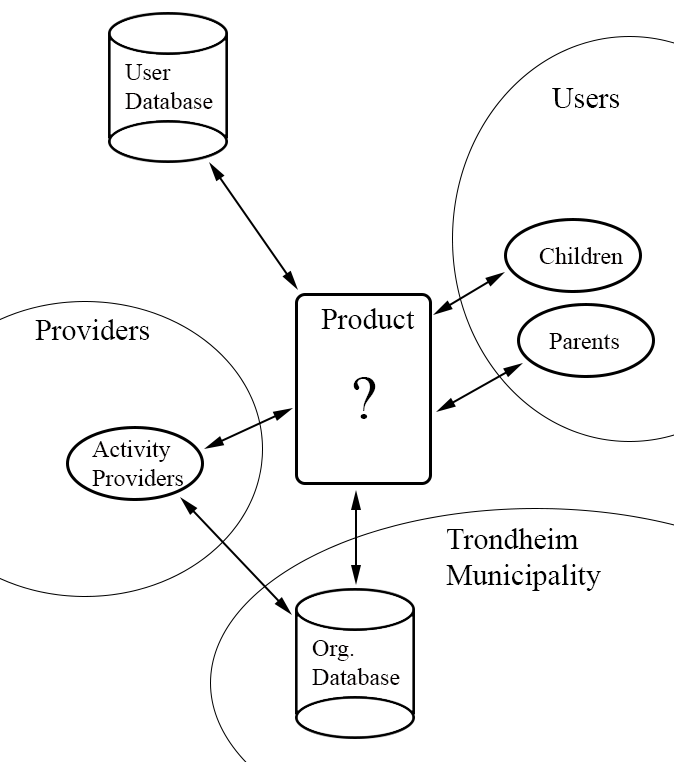
\includegraphics[width=0.5\textwidth]{fig/arkitektur}
\caption{Architecture}
\end{figure}


\section{Back End}

\subsection{Database Structure}
\begin{figure}[h!]
\centering
    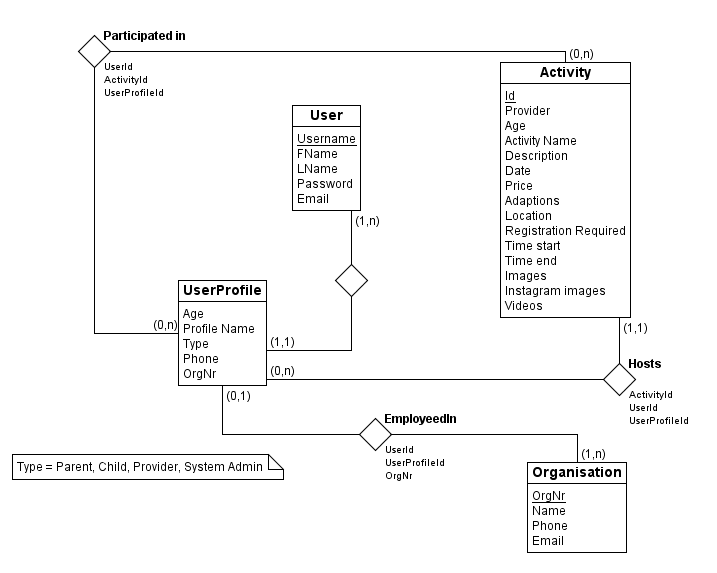
\includegraphics[width=0.85\textwidth]{fig/database_diagram}
\caption{Database structure}
\label{database_figure}
\end{figure}
The database is structured with four different tables; User, UserProfile, Activity and Organisation. These four tables are bounded together by three different relational tables and one single relation between the User table and the UserProfile table. The relational tables are ParticipatedIn, EmployedIn and Hosts (See figure \ref{database_figure}).

The User table is a pre-defined table created by the Django \ref{django} framework. The group chose to use this table to handle User identification. This is a part of Django's security around authentication, and it would be heaps of extra work to write a new secure user authentication system. The group also wanted to devide users into different types of users, and therefor chose to create a UserProfile table which is dependent on the User table. This allowed for customizing user profiles, without tampering with Django's authentication system. 

The rest of the database works like a normal relational database.





\subsection{Access to Aktørbasen}


\section{Front End}

\subsection{Data Flow}

\subsection{Component Diagram}

\subsection{Third Party Interfaces}
In the workshop with the users at the start of the project and during the weekly meetings with the customer, it was often discussed that the web portal should be unique and as easy to use as possible. The users and the customer therefore requested about the opportunity to use third party interfaces like Facebook and Instagram. 
\subsubsection{Facebook API}
From the workshop with the users of skalvi.no, it was mentioned by serveral users that they wanted to be able to log in to the web portal with facebook. 
The customer mentioned that many providers use Facebook to display different activities they offer. 

SKAL SKRIVE MER

the he wanted the opportunity to create new events in the web portal based on existing events on Facebook.  
\subsubsection{Instagram API}
\subsubsection{Log In}

\section{Graphical User Interface}

\subsection{Paper Prototype}
During sprint 0 \ref{sprint0} the group designed a paper prototype as the first design of the application. This was a very helpful asset for the group, as it created a common understanding of what was expected to be developed.  

\subsection{User Interface}

\cleardoublepage